\chapter{The charm-tagged analysis}
    \label{app:CharmTaggedAnalysis}

This appendix reports the main results of the charm-tagged analysis, based on $\unit[20.3]{fb^{-1}}$ of $\pp$ collisions at $\unit[8]{TeV}$.
This analysis has been published in Phys. Rev. D. 90, 052008 (2014) \cite{Aad:2014nra}, together with some of the interpretations of the monojet analysis.
The charm-tagged analysis is presented here for completeness, although it is not strictly part of this Thesis.
This analysis is interpreted in terms of stop pair production with each $\stopone$ decaying as $\stoptocharm$, and complements the exclusion limits of the monojet analysis.

Events are selected with the preselection criteria described in Section~\ref{sec:EventSelection}, with at least four reconstructed jets with $\pt>\unit[30]{GeV}$ and $|\eta|<2.5$.
The kinematics of the charm jets from the stop decays depend mainly on the $\Delta m = m_{\stopone} - m_{\ninoone}$.
As $\Delta m$ decreases, the $\pt$ of the charm jets become softer and it is more likely that other jets from initial state radiation have a higher transverse momentum than the charm jets.
As a consequence, the stop signal is expected to have relatively large jet multiplicities and a jet coming from the hadronization of a charm quark ($c$-tagged) can be found among any of the subleading jets.

Jets are $c$-tagged via a dedicated algorithm using multivariate techniques.
It combines information from the impact parameters of displaced tracks and topological properties of secondary and tertiary decay vertices reconstructed within the jet.
The algorithm provides three probabilities: one targeted for light-flavor quarks and gluon jets ($P_u$), one for charm jets ($P_c$) and one for $b$-quark jets ($P_b$).
From these three probabilities, anti-$b$ and anti-$u$ discriminators are calculated:

\begin{equation}
\begin{split}
\text{anti-}b &\equiv \log{\left(\frac{P_c}{P_b}\right)} \\
\text{anti-}u &\equiv \log{\left(\frac{P_c}{P_u}\right)}.
\end{split}
\label{eq:charmTagDiscriminators}
\end{equation}

These discriminators are then used for the selected jets in the final state.
Figure~\ref{fig:CharmTaggedDiscriminants} shows the distributions of the anti-$b$ and anti-light discriminators for the first- and third-leading jets (ordered in decreasing jet $\pt$), respectively.
The data are compared to MC simulations for the different SM processes, separated by jet flavor, and the multijet processes are estimated following the method described in Appendix~\ref{app:JetSmearingMethod}.
They include the signal preselection defined in Table~\ref{tab:SignalRegionCuts} without applying the tagging requirements.
Good agreement is observed between data and MC simulations.
Two operating points specific to $c$-tagging are used.
The \emph{medium} operating point ($\log{(P_c/P_b)}>-0.9$, $\log{(P_c/P_u)}>0.95$) has a $c$-tagging efficiency of $\approx 20\%$, and a rejection factor of $\approx 8$ for $b$-jets, $\approx 200$ for light-jets and $\approx 10$ for $\tau$-jets.
The \emph{loose} operating point is ($\log{(P_c/P_b)}>-0.9$) has a $c$-tagging efficiency of $\approx 95\%$, with a factor 2.5 rejection of $b$-jets, but with no significant rejection to light or $\tau$ jets.

\begin{figure}[!ht]
  \begin{center}
    \mbox{
      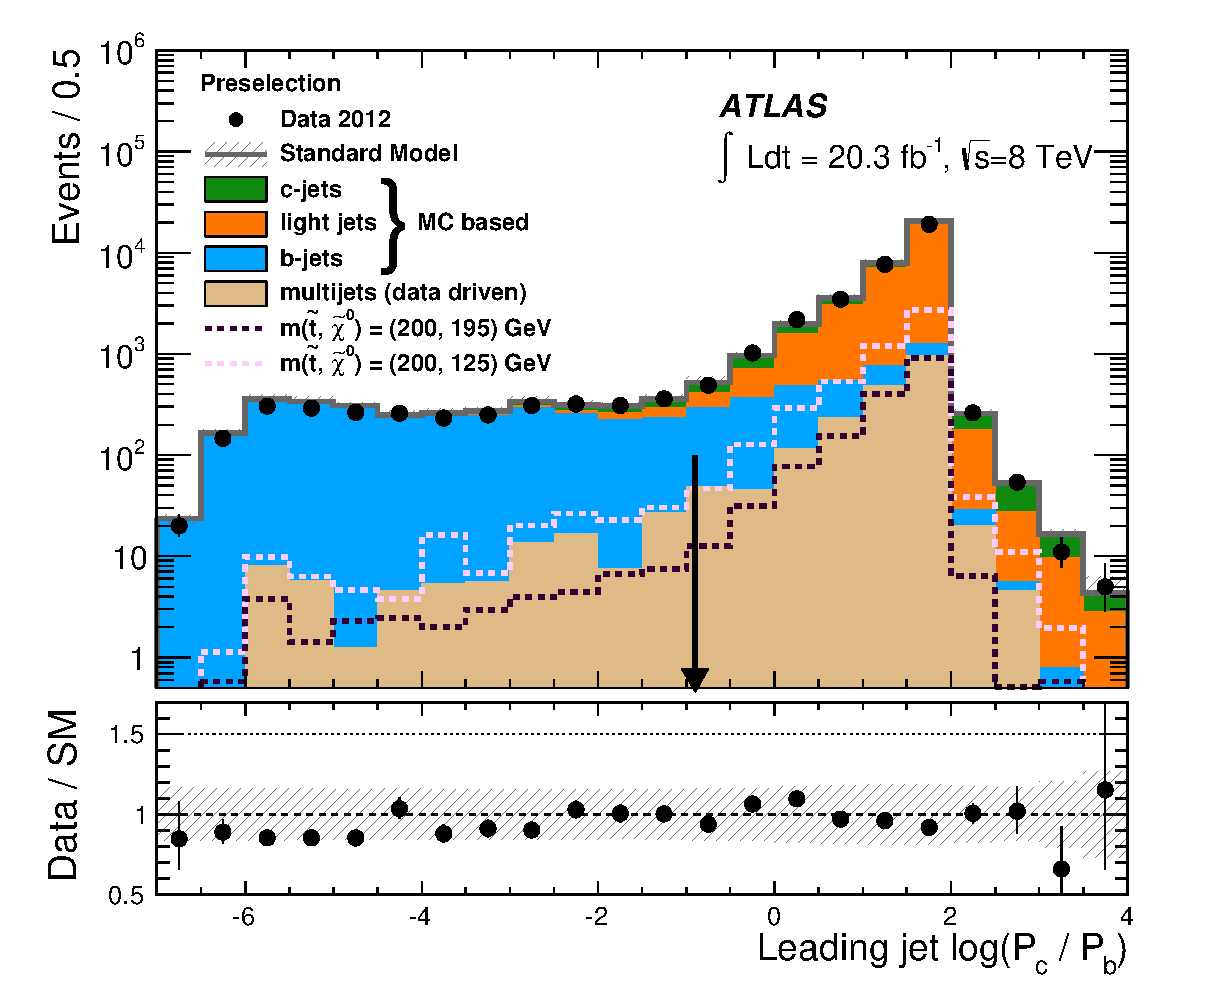
\includegraphics[width=0.495\textwidth]{Appendix_CharmTagged/Figures/can_PreselSRT_jet1logPcPb_final_jetflav.eps}
      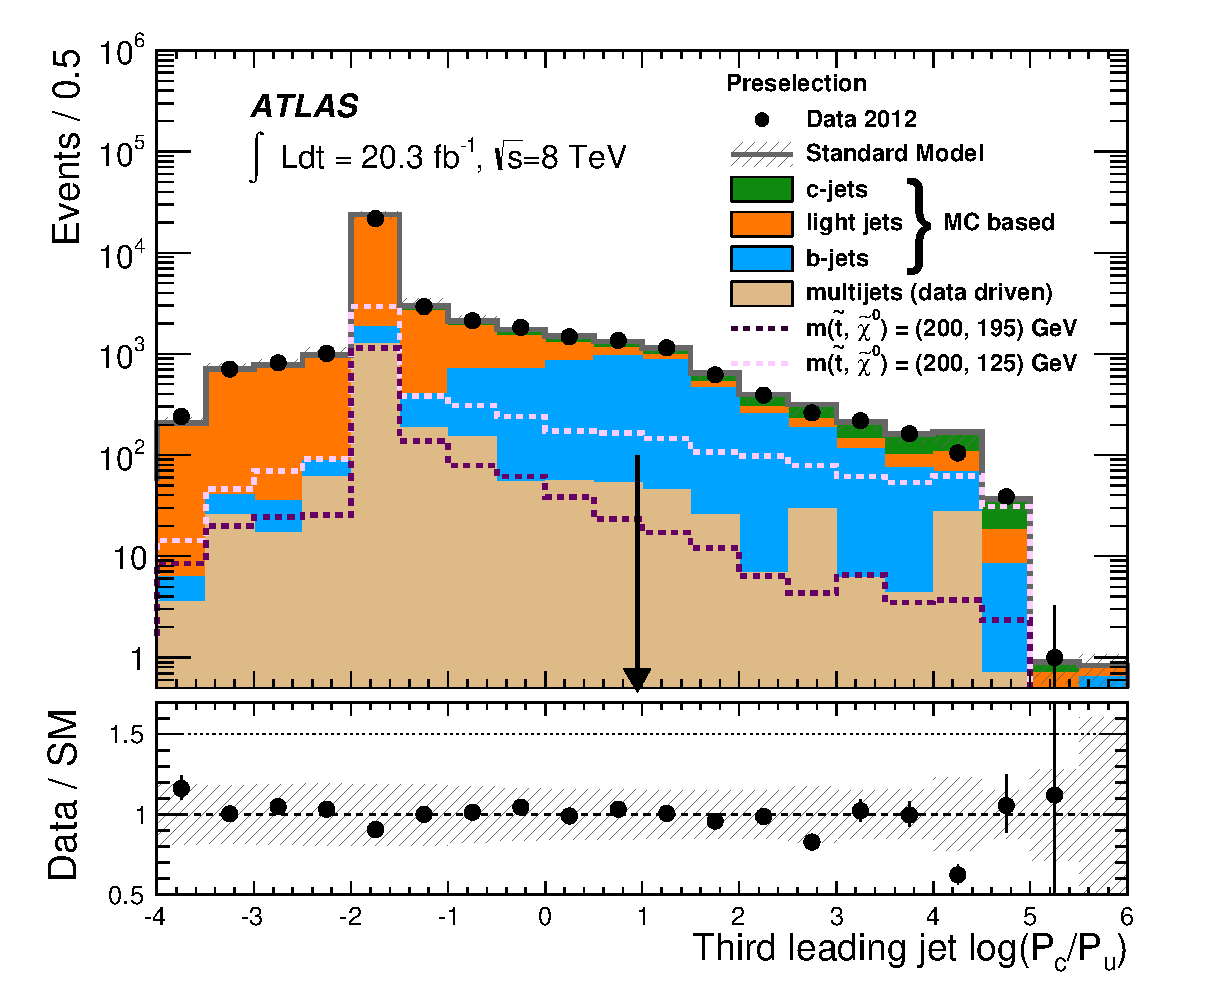
\includegraphics[width=0.495\textwidth]{Appendix_CharmTagged/Figures/can_PreselSRT_jet3logPcPu_final_jetflav.eps}
    }
  \end{center}
  \caption[Distribution of the discriminator against $b$-jets, $\log{(P_c/P_b)}$, for the first-leading jet and against light-jets, $\log{(P_c/P_u)}$, for the third-leading jet.]
{Distribution of the discriminator against $b$-jets, $\log{(P_c/P_b)}$, for the first-leading jet and against light-jets, $\log{(P_c/P_u)}$, for the third-leading jet.
  The data are compared to MC simulations for the different SM processes, separated by jet flavor and include the same signal preselection defined in Table~\ref{tab:SignalRegionCuts} without applying the tagging requirements, which are indicated by the arrows.
  The bottom panels show the ratio between data and MC predictions. The error bands in the ratios include the statistical and experimental uncertainties in the predictions.
  For illustration purposes, the distribution of two different SUSY scenarios for stop pair production are included.
  In the SUSY signal, the first-leading jet mostly originates from ISR and the third-leading jet is expected to contain a large fraction of $c$-jets.}
  \label{fig:CharmTaggedDiscriminants}
\end{figure}

A veto against $b$-jets is applied to the selected jets in the event by using a loose $c$-tag requirement.
In addition, at least one of the three subleading jets is required to be $c$-tagged using the medium criteria.
The leading jet is required to have $\pt>\unit[290]{GeV}$ and two separate signal regions, C1 and C2, are defined with $\met>\unit[250]{GeV}$ and $\met>\unit[350]{GeV}$, respectively.
The tighter requirements on $\met$ for C2 targets models with larger stop and neutralino masses.
Table~\ref{tab:CharmTaggedSignalRegionCuts} summarizes the C1 and C2 signal region cuts.

\begin{table}[!t]
  \renewcommand{\baselinestretch}{1}
  \begin{center}
    \begin{small}
      \begin{tabular*}{\textwidth}{@{\extracolsep{\fill}}lcc}\hline\hline
        \multicolumn{3}{c}{\small{\textbf{Selection criteria}}} \\\hline
        %%% --- PRESELECTION
        \multicolumn{3}{c}{{\small{Preselection}} } \\\hline
        \multicolumn{3}{l}{Primary vertex}\\
        \multicolumn{3}{l}{$\met > 150$~GeV }\\
        \multicolumn{3}{l}{At least one jet with $\pt >150$~GeV and $|\eta|< 2.8$}\\
        \multicolumn{3}{l}{Jet quality requirements}   \\
        \multicolumn{3}{l}{Lepton vetoes}\\ \hline
        %%%% --- MONOJET
        %\multicolumn{7}{c}{\small{Monojet-like selection}}\\\hline
        %\multicolumn{7}{l}{At most a total of three jets with $\pt > 30$~GeV and $|\eta|<2.8$}\\
        %\multicolumn{7}{l}{$\Delta\phi(\text{jet}, \mathbf{p_{T}}^\text{miss}) > 0.4$}\\\hline
        %Signal region                   & M1  & M2  & M3  & M4  & M5  & M6  \\
        %Minimum leading jet $\pt$ (GeV) & 280 & 340 & 450 & 450 & 550 & 600 \\
        %Minimum $\met$ (GeV)            & 220 & 340 & 450 & 340 & 550 & 600 \\ \hline
        %%% --- C-TAGGED
        \multicolumn{3}{c}{\small{$c$-tagged selection}}\\\hline
        \multicolumn{3}{l}{At least a total of four jets with $\pt > 30$~GeV and $|\eta|<2.5$}\\
        \multicolumn{3}{l}{$\Delta\phi(\text{jet}, \mathbf{p_{T}}^\text{miss}) > 0.4$}\\
        \multicolumn{3}{l}{All four jets must pass loose tag requirements ($b$-jet vetoes)}\\
        \multicolumn{3}{l}{At least one medium charm tag in the three subleading jets}\\\hline
        Signal region        & C1 & C2   \\
        Minimum leading jet $\pt$ [GeV] & 290 & 290   \\
        Minimum $\met$ [GeV] & 250 & 350  \\ \hline\hline
      \end{tabular*}
    \end{small}
  \end{center}
  \caption[Event selection criteria applied for the signal regions of the charm-tagged analysis.]{Event selection criteria applied for the signal regions of the charm-tagged analysis.}
  \label{tab:CharmTaggedSignalRegionCuts}
\end{table}

The expected SM background for this analysis is dominated by $\znn$, $\ttbar$ and $\wln$ production, including smaller contributions from $\zll$, single-top, diboson ($WW$, $WZ$, $ZZ$) and multijet processes.

The $W/Z$ + jets processes are estimated in control regions, defined with close cuts as those from the monojet approach, with differences motivated by the background composition and the contribution from heavy-flavor jets.
A tighter cut of $\unit[81]{GeV} < m_{\mu\mu} < \unit[101]{GeV}$ is used to define the $\zmm$ + jets control sample, to further reject $\ttbar$ contamination.
This region is complemented with $\zee$+jets control sample, with the same requirements in the invariant mass, with the calorimeter clusters associated to electrons removed from the $\met$.
As in the monojet case, control samples for $\wen$+jets and $\wmn$+jets are also defined.
Due to the reduction in the statistics as a consequence of the application of the $c$-tagging, the $\met$ and leading jet $\pt$ requirements are lowered to $\unit[150]{GeV}$.

The $\ttbar$ process is estimated with a dedicated control region selecting two opposite-charge leptons ($ee$, $\mu\mu$ or $e\mu$ configurations), the same selection criteria for jet multiplicity and $c$-tagging as in the signal region, and relaxed $\met>\unit[150]{GeV}$ and leading jet $\pt>\unit[150]{GeV}$.

\begin{figure}[!ht]
  \begin{center}
    \mbox{
      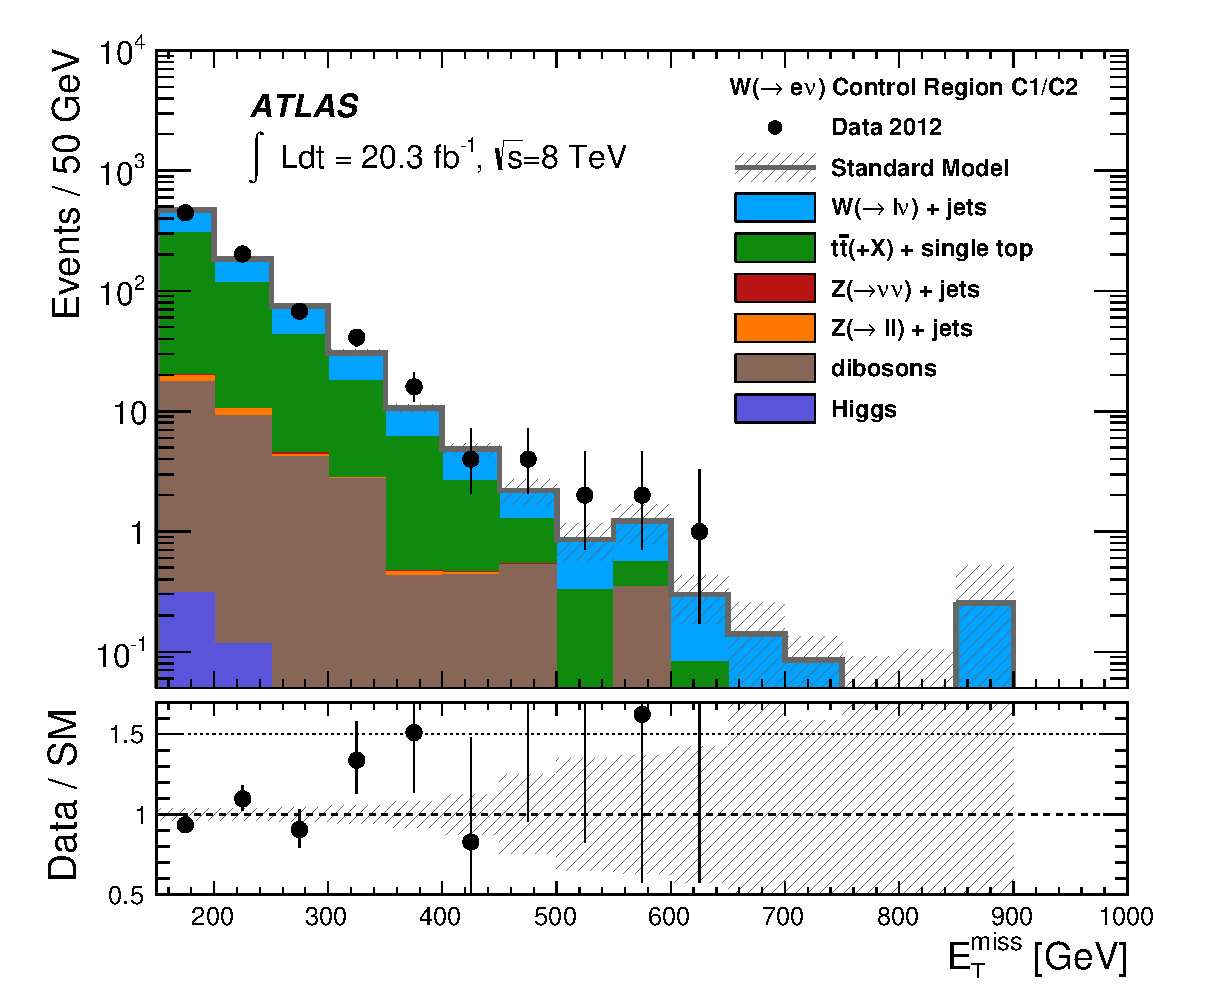
\includegraphics[width=0.495\textwidth]{Appendix_CharmTagged/Figures/can_VR_Wenu_C1_met_final.eps}
      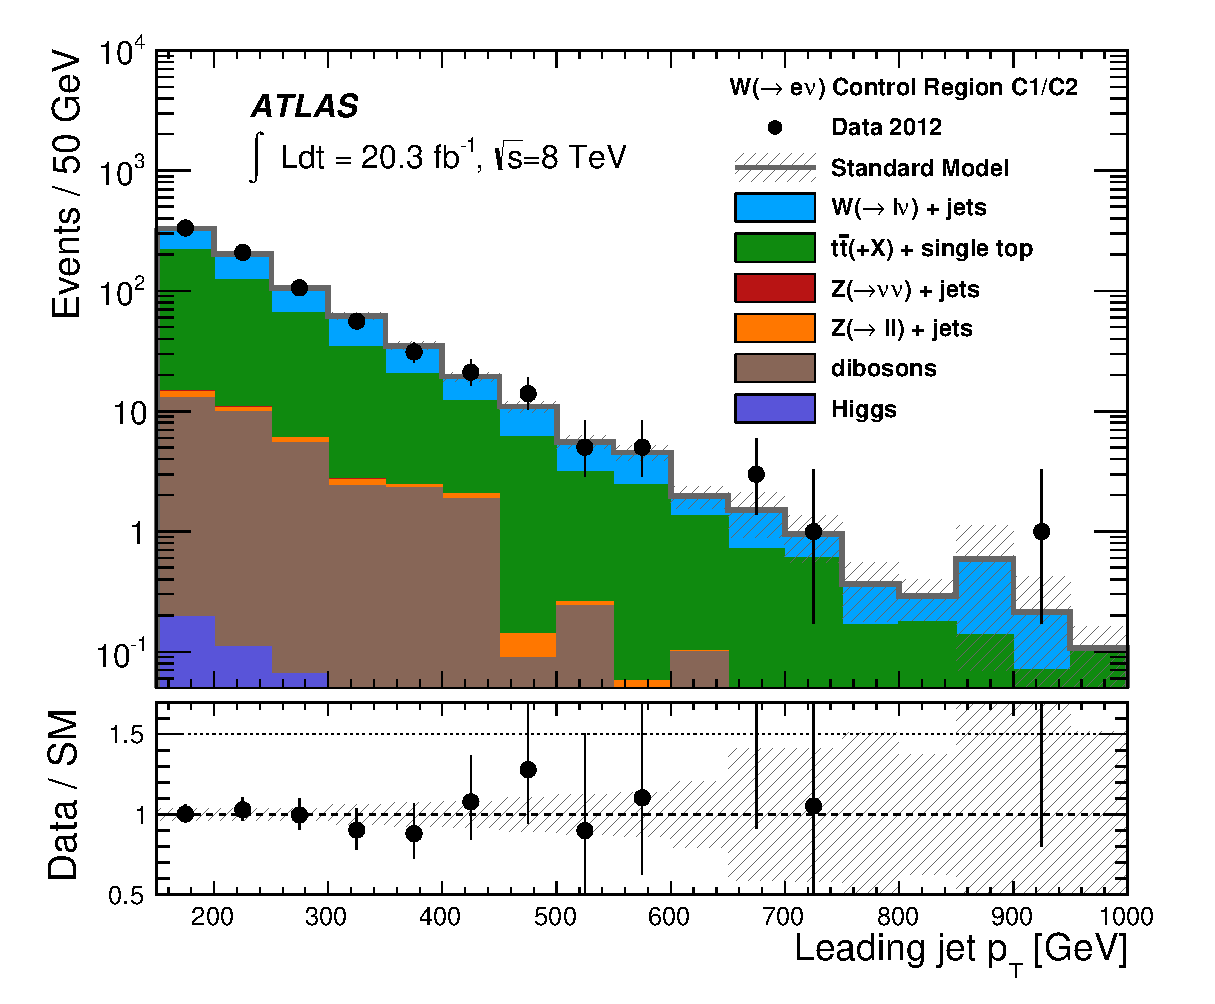
\includegraphics[width=0.495\textwidth]{Appendix_CharmTagged/Figures/can_VR_Wenu_C1_jet1PtWithEle_final.eps}
    }
    \mbox{
      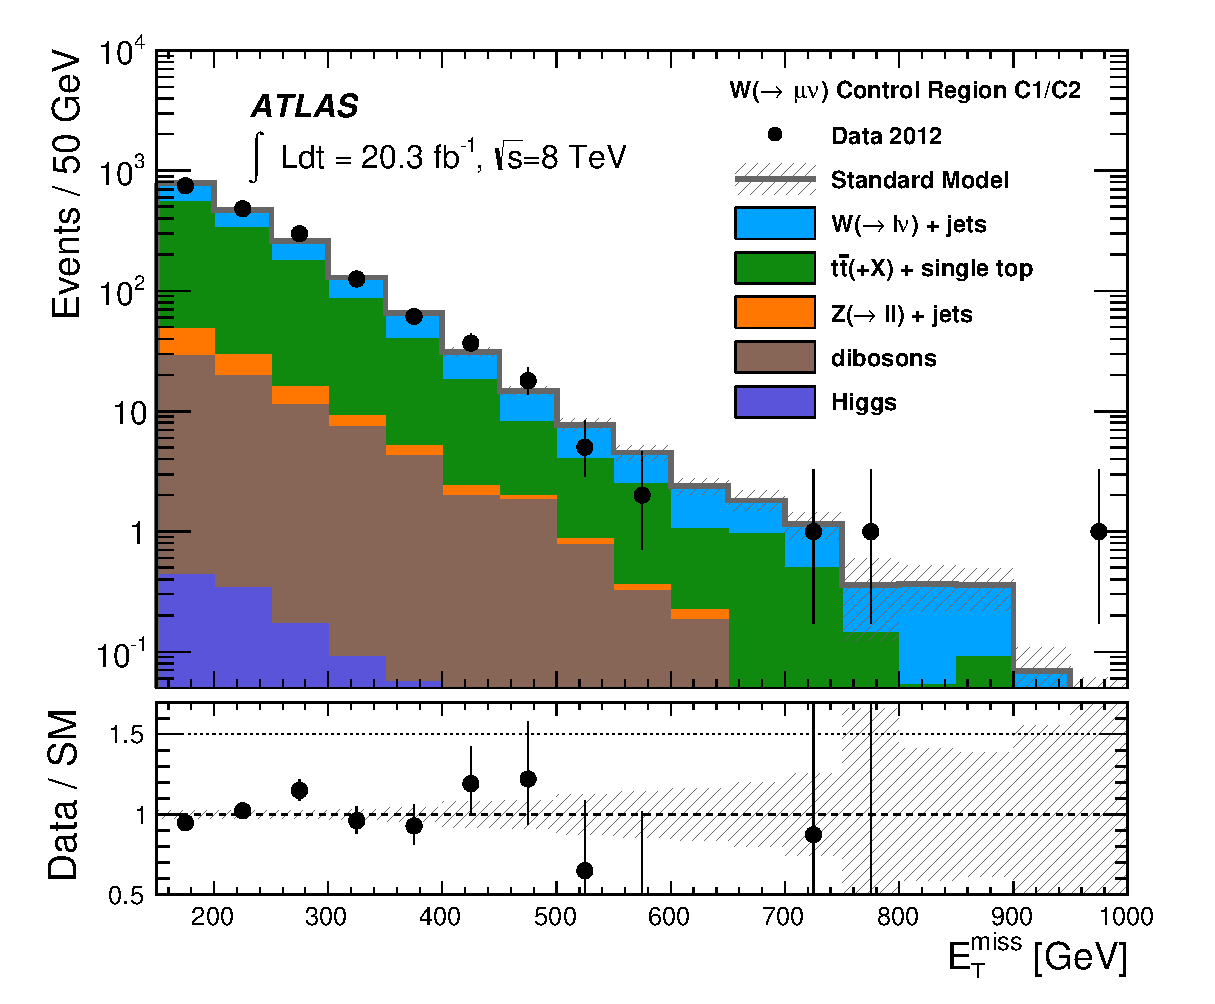
\includegraphics[width=0.495\textwidth]{Appendix_CharmTagged/Figures/can_VR_Wmunu_C1_metnomu_final.eps}
      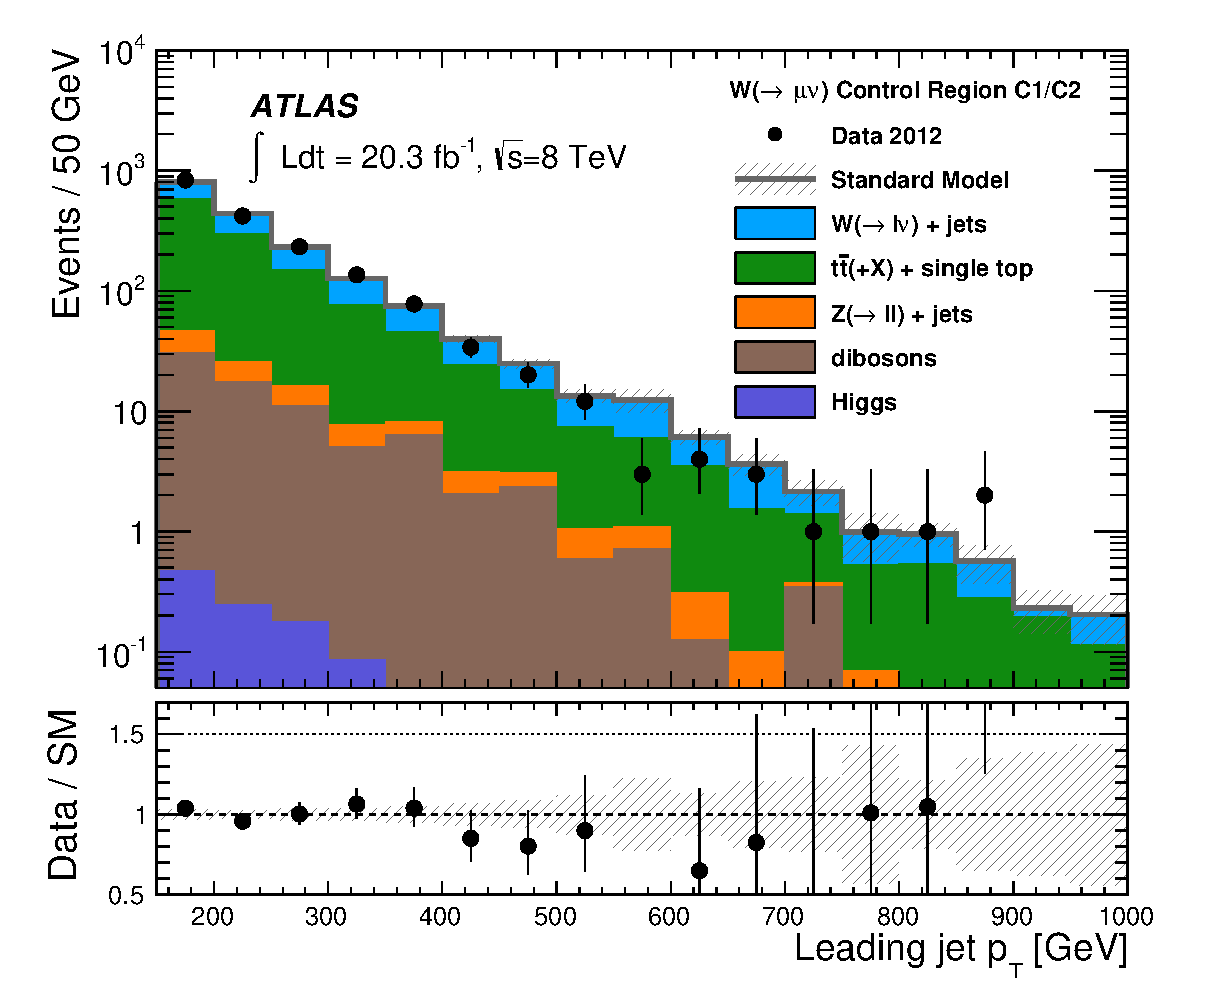
\includegraphics[width=0.495\textwidth]{Appendix_CharmTagged/Figures/can_VR_Wmunu_C1_jet1Pt_final.eps}
    }
    \mbox{
      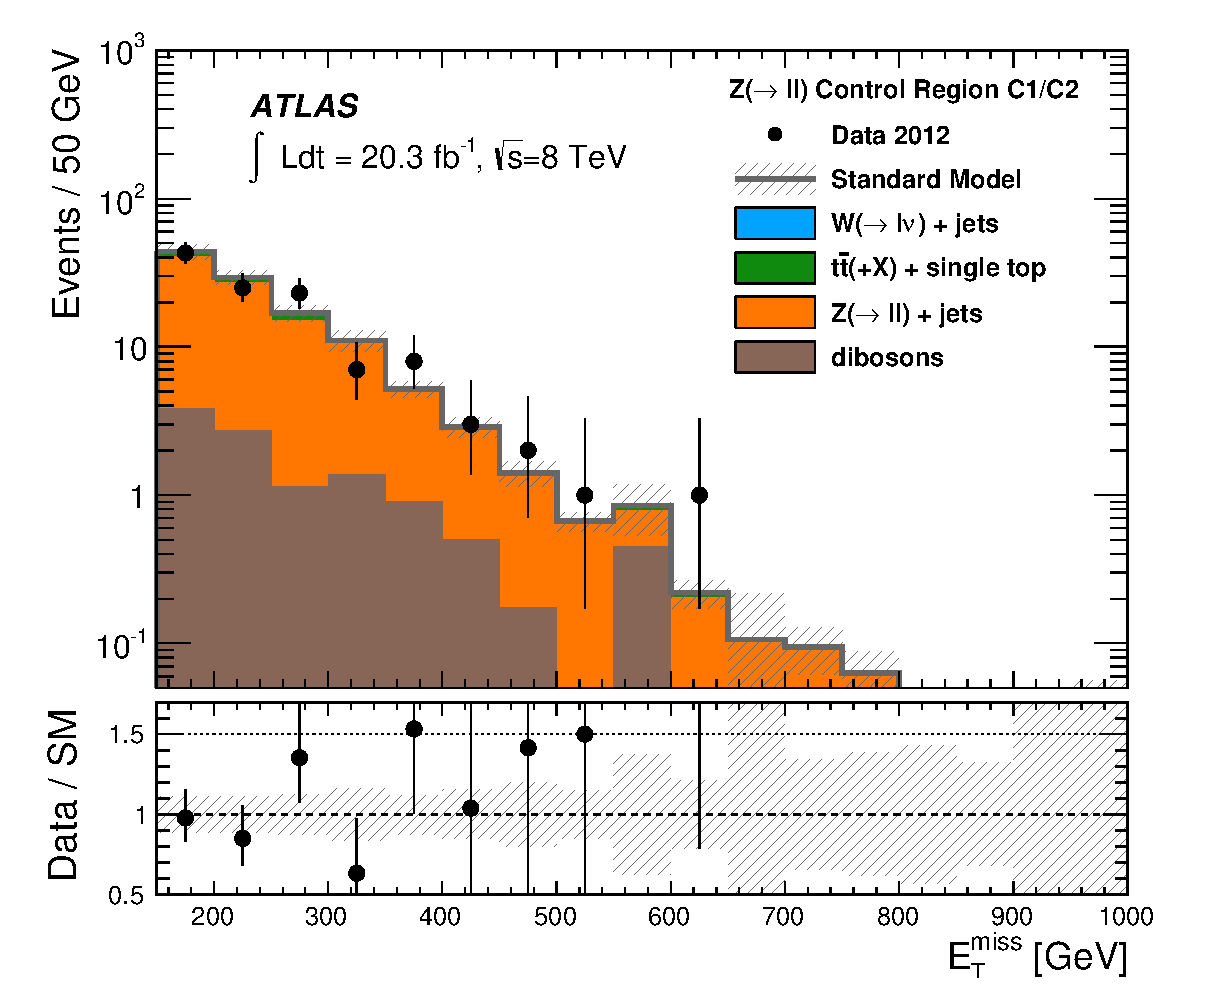
\includegraphics[width=0.495\textwidth]{Appendix_CharmTagged/Figures/can_VR_Zll_C1_metnolep_final.eps}
      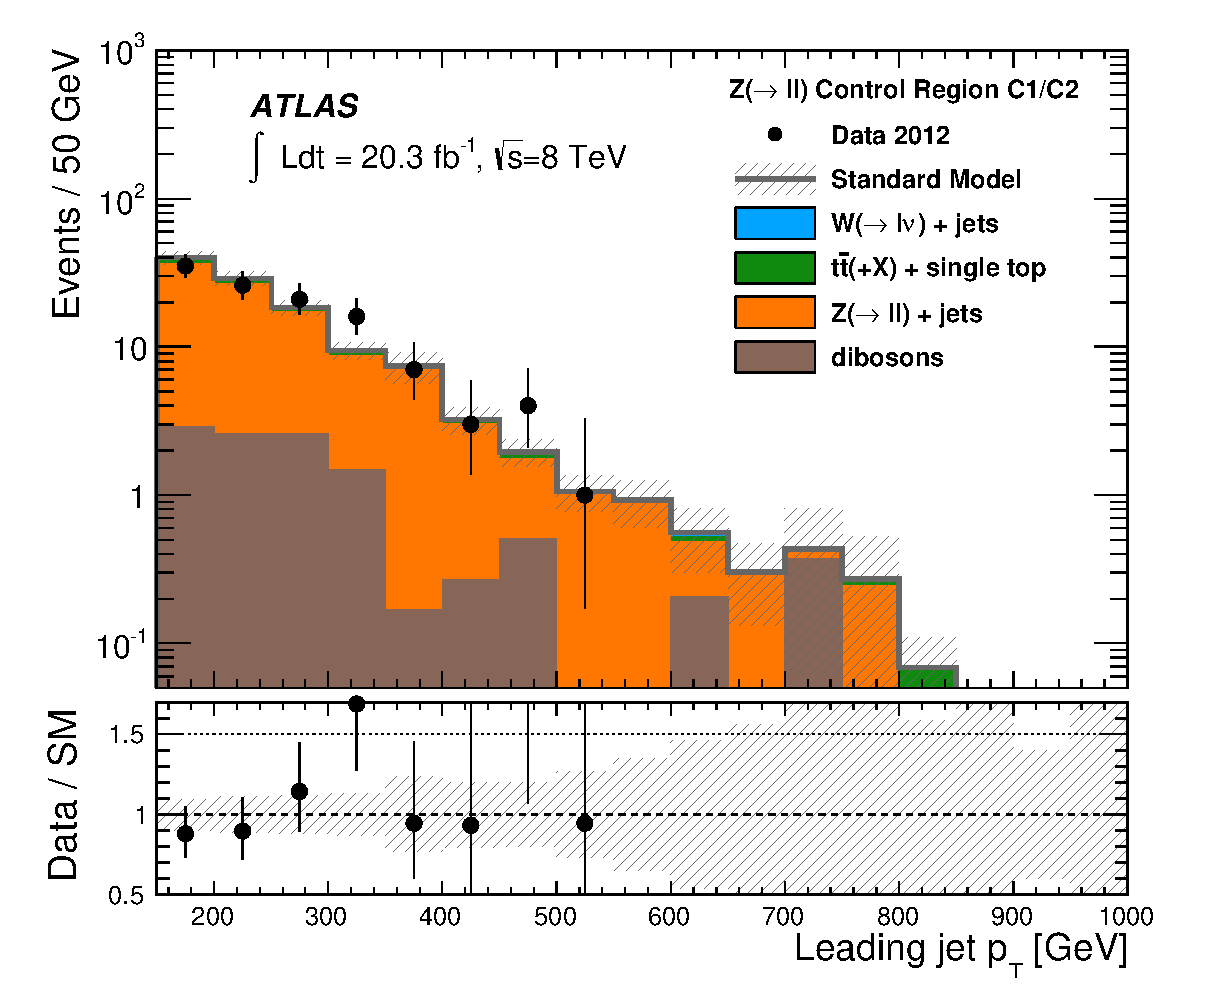
\includegraphics[width=0.495\textwidth]{Appendix_CharmTagged/Figures/can_VR_Zll_C1_jet1Pt_final.eps}
    }
  \end{center}
  \caption[$\met$ and leading jet $\pt$ distributions in the $\wen$+jets, $\wmn$+jets and $\zll$+jets control regions, after the normalization factors extracted from the fit have been applied.]{The measured $\met$ and leading jet $\pt$ distributions in the $\wen$+jets, $\wmn$+jets and $\zll$+jets control regions compared to the background predictions. The latter include the global normalization factors extracted from the fit. The error bands in the ratios include the statistical and experimental uncertainties on the background predictions.}
  \label{fig:Plot_CharmTagged_EW_Jetkinematics}
\end{figure}


\begin{figure}[!ht]
  \begin{center}
    \mbox{
      \includegraphics[width=0.495\textwidth]{Appendix_CharmTagged/Figures/can_VR_TTBarll_C1_metnomu_final.eps}
      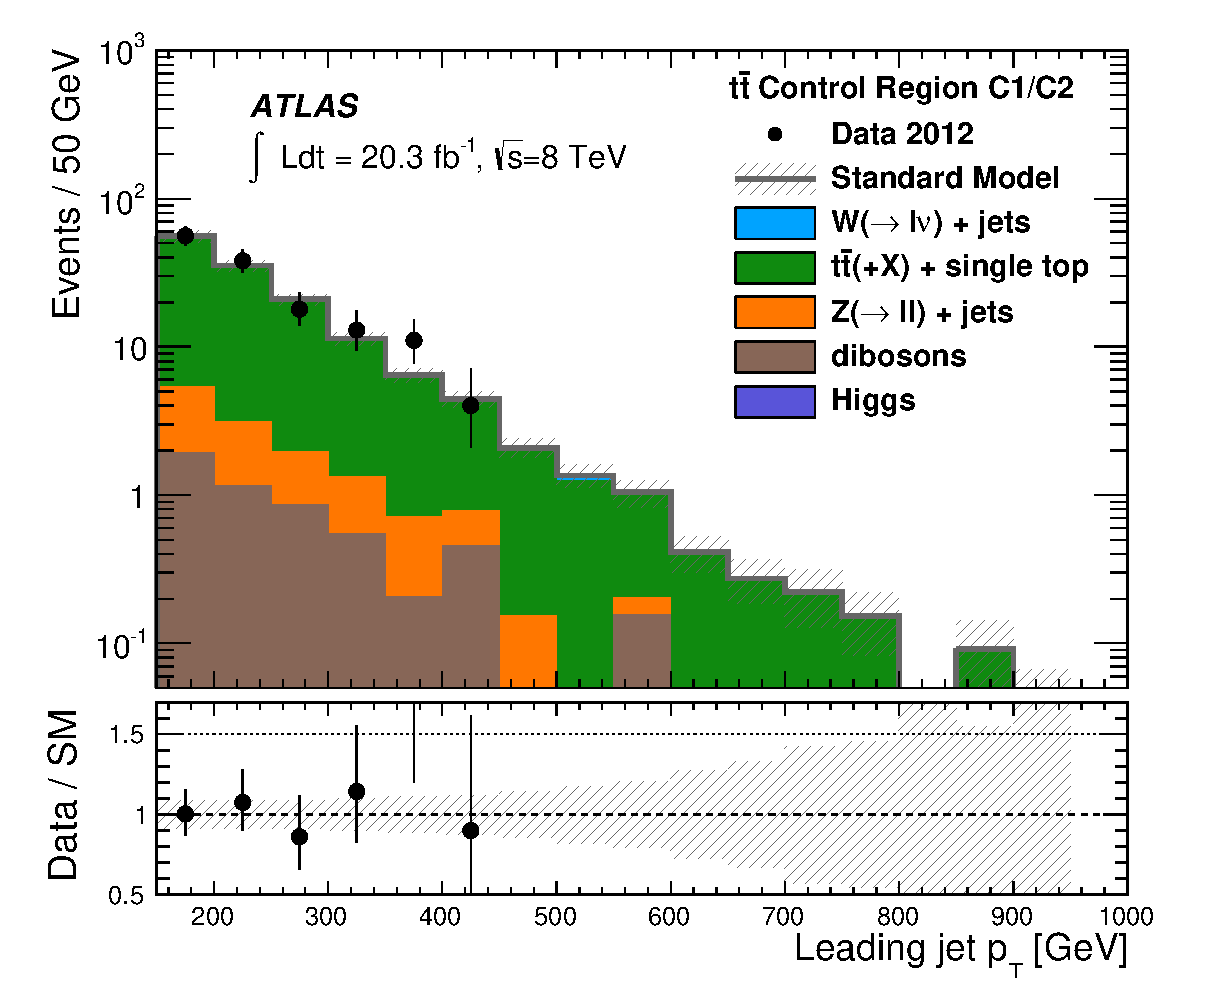
\includegraphics[width=0.495\textwidth]{Appendix_CharmTagged/Figures/can_VR_TTBarll_C1_jet1PtWithEle_final.eps}
    }
  \end{center}
  \caption[$\met$ and leading jet $\pt$ distributions in the $\ttbar$ control region for the charm-tagged selection, after the normalization factors extracted from the fit have been applied.]{The measured $\met$ and leading jet $\pt$ distributions in the $\ttbar$ control region compared to the background predictions. The latter include the global normalization factors extracted from the fit. The error bands in the ratios include the statistical and experimental uncertainties on the background predictions.}
  \label{fig:Plot_CharmTagged_ttbar_Jetkinematics}
\end{figure}


A simultaneous likelihood fit to the $\wen$+jets, $\wmn$+jets, $\zll$+jets and $\ttbar$ control samples is performed following the techniques described in Section~\ref{sec:Fit}.
After the fit, the $W/Z$+jets backgrounds receive a multiplicative correction between 0.8 and 0.9 while the $\ttbar$ is normalized with a scale factor of 1.1.

The data and the expected background predictions for the signal regions C1 and C2 are summarized in Table~\ref{tab:CharmTaggedSignalRegions}.
Good agreement is observed between data and MC predictions.
These predictions are determined with a total uncertainty of 10\% and 14\%, respectively.
Figure~\ref{fig:Plot_CharmTagged_SR_Jetkinematics} shows the measured leading jet $\pt$ and $\met$ distributions compared to the background predictions.
For illustration purposes, the distribution of two different SUSY scenarios for stop pair production in the $\stoptocharm$ decay channel with stop masses of $\unit[200]{GeV}$ and neutralino masses of $\unit[125]{GeV}$ and $\unit[195]{GeV}$ are included.

\begin{table}[!ht]
\begin{center}
\begin{small}
\begin{tabular*}{\textwidth}{@{\extracolsep{\fill}}lrr}\hline
{\bf  Signal Region}  & \textbf{C1} & \textbf{C2}  \\
    Observed events  (20.3 fb${}^{-1}$)&  $208$  & $71$  \\ \hline

    SM prediction &  $210 \pm 21$  & $75 \pm 11$ \\ \hline

    $\wen$        &  $11 \pm 2$ &  $3.0 \pm 0.7$ \\

    $\wmn$        &  $8 \pm 2$ &  $3.0 \pm 0.7$  \\

    $\wtn$        &  $42 \pm 9$  & $14 \pm 3$ \\

    $\zee$        &  $-$   &  $-$ \\

    $\zmm$        &  $0.07 \pm 0.01$  & $0.04 \pm 0.01$  \\

    $\ztt$        &  $0.7 \pm 0.1$    & $0.15 \pm 0.03$ \\

    $\znn$        &  $62 \pm 9$ & $27 \pm 3$  \\

    $\ttbar$, single top          &     $63 \pm 13$   &  $18 \pm 4$ \\

    Dibosons      &  $21 \pm 13$  & $10 \pm 9$  \\

    Higgs         &  $0.16 \pm 0.03$  & $0.07 \pm 0.01$  \\

    Multijets     &  $2 \pm 2$  & $0.1 \pm 0.1$  \\ \hline \hline

    \end{tabular*}
    \end{small}

    \end{center}
    \caption[Data and background predictions in the signal regions C1 and C2.]{Data and background predictions in the signal regions C1 and C2.
      For the SM predictions both statistical and systematic uncertainties are included.
        Note that in each case the individual
        uncertainties can be correlated, and do not necessarily add up quadratically to the total background uncertainty.
    }
\label{tab:CharmTaggedSignalRegions}
\end{table}

\begin{figure}[!ht]
  \begin{center}
    \mbox{
      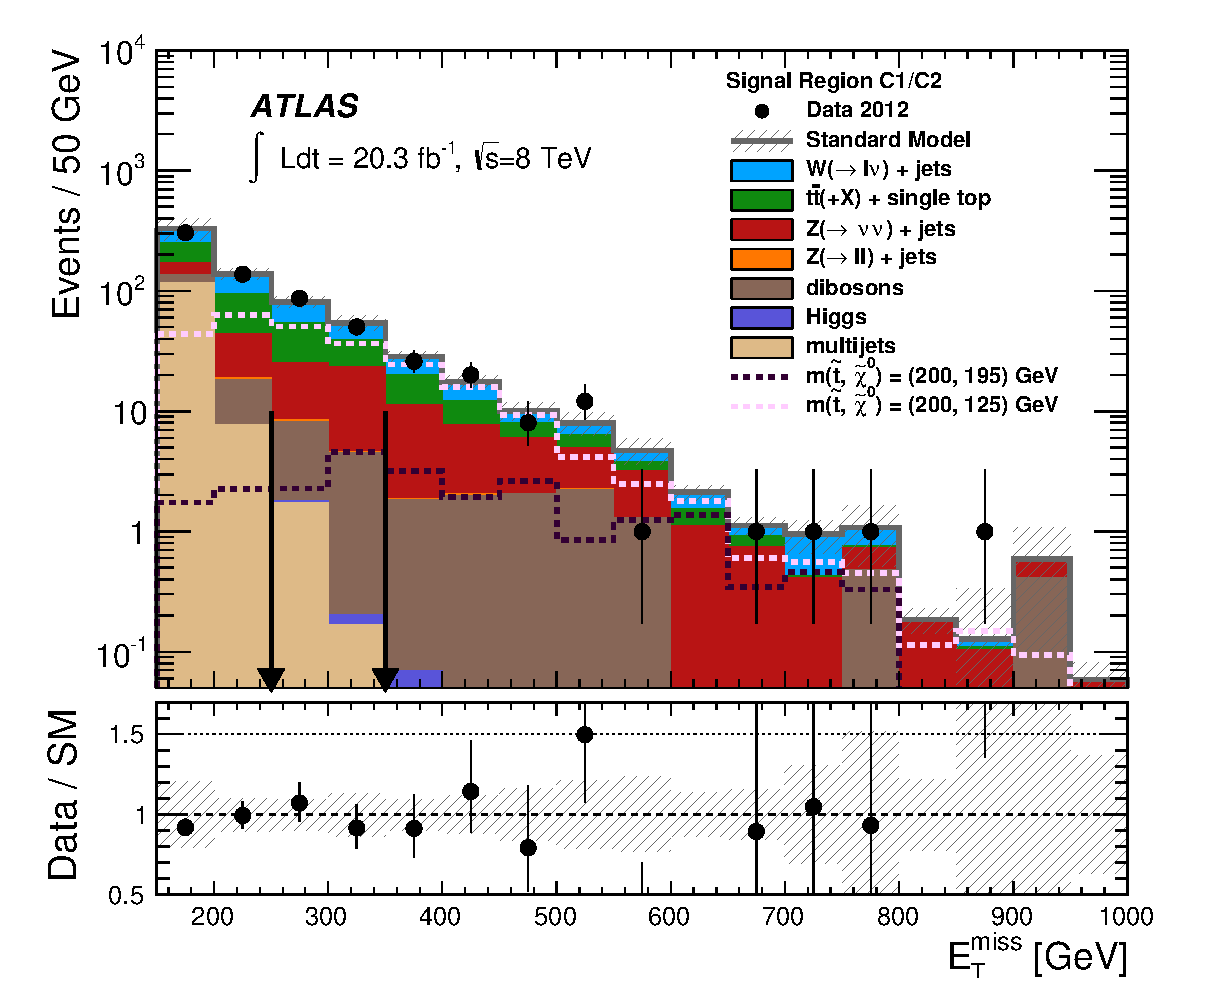
\includegraphics[width=0.495\textwidth]{Appendix_CharmTagged/Figures/can_SR_C1NoMet_met_final.eps}
      \includegraphics[width=0.495\textwidth]{Appendix_CharmTagged/Figures/can_SR_C1NoJetPt_jet1Pt_final.eps}
    }
    \mbox{
      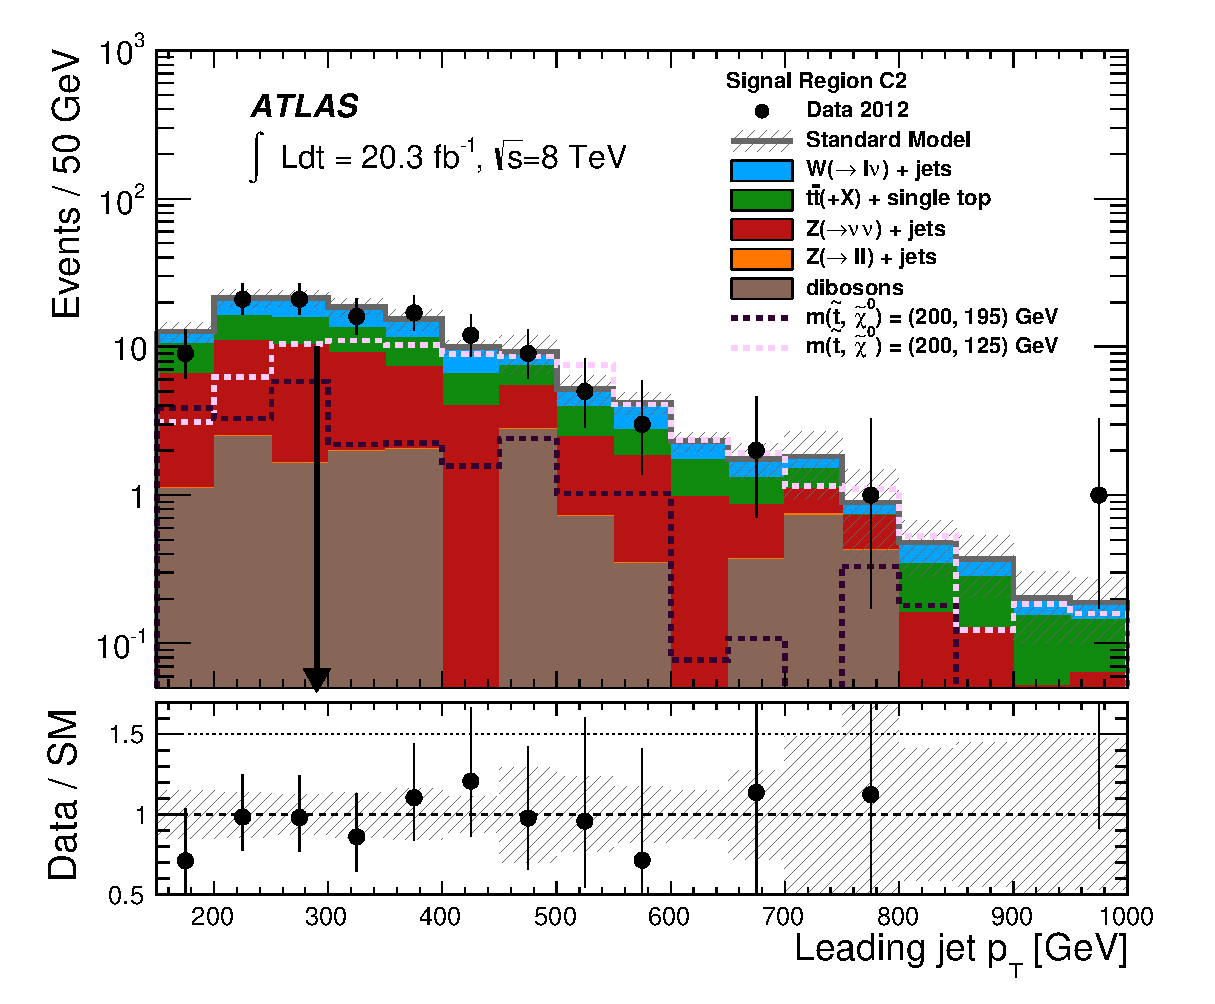
\includegraphics[width=0.495\textwidth]{Appendix_CharmTagged/Figures/can_SR_C2NoJetPt_jet1Pt_final.eps}
      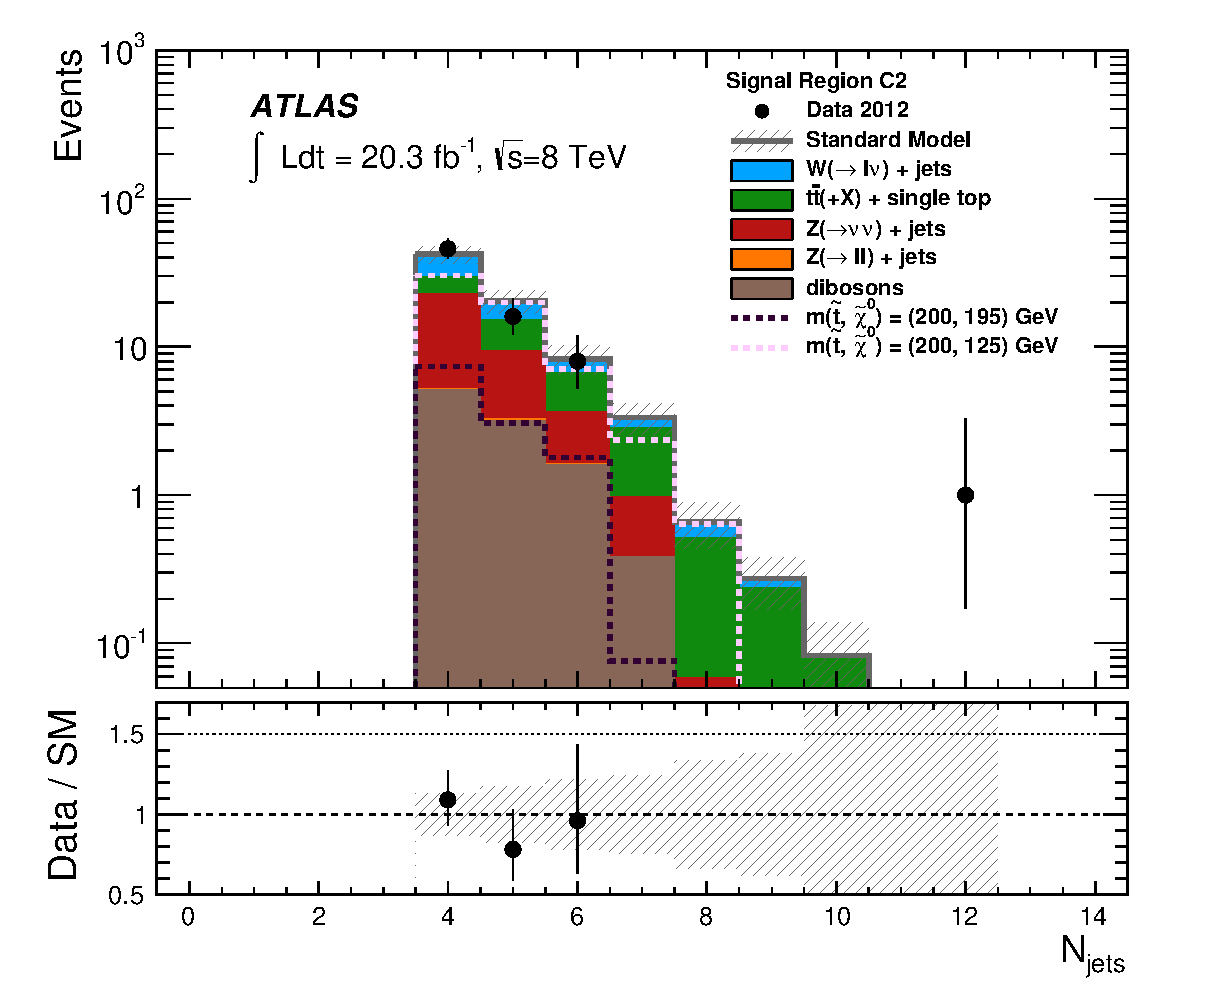
\includegraphics[width=0.495\textwidth]{Appendix_CharmTagged/Figures/can_VR_SRC2_nJet30_final.eps}
    }
  \end{center}
  \caption[Several kinematic distributions in the C1 and C2 signal regions for the charm-tagged analysis.]{(top) Measured $\met$ and leading jet $\pt$ distributions for the C1 selection before the cut in the variable shown (as indicated by the vertical arrows) is applied. In the case of the $\met$ distribution, the cuts corresponding to C1 and C2 selections are both indicated.
  (bottom) Measured leading jet $\pt$ and jet multiplicity for the C2 selection. The data are compared to the SM predictions. For illustration purposes, the distribution of two different SUSY scenarios are included. The error bands in the ratios include both the statistical and systematic uncertainties on the background predictions.}
\label{fig:Plot_CharmTagged_SR_Jetkinematics}
\end{figure}

These results are translated to exclusion limits on the pair production of top squarks with $\stoptocharm$ (BR=100\%) as a function of the stop mass for different neutralino masses.
Expected and observed exclusion limits are extracted following the $CL_s$ technique described in Chapter~\ref{chapter:StatisticalModel}, for which a simultaneous fit to the signal and control regions is performed including statistical and systematic uncertainties.

Figure~\ref{fig:ExclusionStoptocharmCharmTagged} shows the 95\% CL exclusion limits for the (best expected) combination of the signal regions C1 and C2. 
The 95\% CL observed limits corresponding to the $\pm 1 \sigma$ variations on the SUSY theoretical cross sections are also added.
The charm-tagged analysis excludes the masses of the stop up to 270~GeV when $\Delta m$ is large.
The sensitivity of the analysis reduces when the $\Delta m$ decreases, due to the c-tagging requirements in the selection.
For compressed mass configurations, the charm jets are too soft to be identified and therefore, only stop masses up to 180~GeV can be excluded.

\begin{figure}[!ht]
\begin{center}
\mbox{
\includegraphics[width=0.795\textwidth]{Appendix_CharmTagged/Figures/limitPlotStop_Stop_combined_C1_C2_.eps}
}
\end{center}
\caption[Exclusion plane at 95\% CL for stop pair production with $\stoptocharm$ as a function of the $m_{\stop}$ and $m_{\ninoone}$]{Exclusion plane at 95\% CL as a function of stop and neutralino masses. The observed (red line) and expected (blue line) upper limits from this analysis are compared to previous results from Tevatron experiments~\cite{Abazov:2008rc}, and from LEP experiments~\cite{Aaltonen:2012tq} at CERN with squark mixing angle $\theta=0^{\circ}$. The dotted lines around the observed limit indicate the range of observed limits corresponding to $\pm 1 \sigma$ variations on the NLO SUSY cross section predictions. The shaded area around the expected limit indicates the expected $\pm 1 \sigma$ ranges of limits in the absence of a signal. A band for $m_{\stopone} - m_{\ninoone}< \unit[2]{GeV}$ indicates the region in the phase space for which the stop can become long-lived \protect\cite{Aad:2014nra}.}
\label{fig:ExclusionStoptocharmCharmTagged}
\end{figure}
